% Author - Jon Arnt Kårstad, NTNU IMT
\documentclass{article}

% Importing settings from our file "setup.sty"
\usepackage{setup}

% package for acronyms and description of words
% https://www.overleaf.com/learn/latex/glossaries
\usepackage[acronym]{glossaries}

\usepackage{cleveref}
\usepackage{xurl}

\definecolor{code}{HTML}{eeeeee}
\setminted{mathescape,
               escapeinside=||,
               linenos,
               numbersep=5pt,
               autogobble,
               frame=lines,
               framesep=2mm,
               bgcolor=code,
               breaklines=true,
               }

% Beginning of document
\begin{document}

% Inserting title page
\import{./}{title}


% Defining front matter settings (Norsk: innstillinger for forord m.m.)
\frontmatter

\section*{Abstract}
This is considered the end result of the semester project in the course TFE4152 Design of Integrated Circuits, at NTNU.\\
This report includes the applied theory and the design process of a CMOS implementation of the digital control circuit as well as the analog readout circuit for a four pixel digital camera.\\
The report is intended for readers with knowledge within electrical engineering and/or CMOS technology, but the basic concepts could be understood by anyone.\\
The simulation verifies the intended functionality of both the analog and digital part of the camera, but has yet to simulated together in a mixed signal simulation as well as being implemented and tested in actual hardware. 

All source code and the source of this document can also be found in out GitHib reposiory. 

\url{https://github.com/oyvindskaaden/TFE4152-DIC-Project}.

\clearpage

% Inserting table of contents
\tableofcontents

\clearpage
% Inserting list of figures & list of tables
\listoffigures
\listoftables

% Defining main matter settings (Norsk: innstillinger for hoveddelen av teksten)
\mainmatter

% Introduction explaining this LaTeX-template
\section*{Abbreviations}

\begin{tabular}{l c l}
CMOS &  & Complimentary metal-oxide-semiconductor \\
HDL &  & Hardware Description Language \\
SPICE & & Simulation Program with Integrated Circuit Emphasis \\
NMOS & & N-channel metal-oxide-semiconductor \\
PMOS & & P-channel metal-oxide-semiconductor \\
FF & & Fast Fast, process corner in CMOS production\\
SS & & Slow Slow, process corner in CMOS production\\
SF & & Slow Fast, process corner in CMOS production\\
FS & & Fast Slow, process corner in CMOS production\\
TT & & Typical Typical, process corner in CMOS production\\
ADC & & Analog to Digital Converter\\
VLSI & & Very Large Scale Integration\\
FSM & & Finite State Machine\\
FET &  & Field Effect Transistor \\
\end{tabular}

\clearpage

\clearpage
\section{Introduction}
To capture digital representations of images digital cameras are used. 
As these cameras are becoming more advanced while reproducing better images, they are still required to shrink in physical size.\\
CMOS technology can be a solution to the challenges faced when shrinking physical size while increasing the performance. \\

This project report completes a theoretical CMOS implementation of a digital camera, with both an analog readout circuit and a digital control module.
The analog circuit is simulated and verified using SPICE simulations, while the digital is implemented using the HDL SystemVerilog. 


\clearpage
\newpage
\section{Theory}
\label{Theroy}
The objective of this chapter is to introduce the reader to the applied theory that is needed for the implementation of a readout- and controll circuit for a digital camera.

\subsection{Field effect transistors}
\label{FET}
Field effect transistors are a fundamental building block of modern electronics design. 
As they are able to be produced quite small, they are by far the most used components in integrated circuit design. 
This is also due to the fact that they are versatile and suitable for alot of applications such as signal amplification and digital logic \cite{sedra_smith_2016}.\\
The most common type of FETs are NMOS and PMOS. 
These are transistors created by silicone dioxide, where the substrate, two heavily doped regions, and a gate electrode creates the device terminals. 
For NMOS the substrate is of p-type and the terminals are made up of n-doped regions. 
The opposite is true for PMOS, n-type substrate and p-doped regions make up the terminals. 
This similar structure with opposite regions, make the NMOS and PMOS complimentary as the polarities are opposite of eachother \cite{sedra_smith_2016}.


\subsubsection{CMOS}
\label{CMOS}
Complementary MOS (CMOS) is a technology that uses both NMOS and PMOS transistors to create digital and analog integrated circuits. 
CMOS is the most widely used IC technology, as it has taken over many applications that for a long time, only were possible by bipolar devices. As well as the previously mentioned versatility \cite{sedra_smith_2016}. 

As mentioned in \cref{FET} transistors are made up of heavily doped regions and a gate electrode. 
To induce a channel in a PMOS transistor, a negative voltage with a higher magnitude than a threshold needs to be applied to the gate terminal. 
This forms a current channel between the source and drain terminal \cite{sedra_smith_2016}.\\
The condition can be described as:
\begin{equation}
    |V_{gs}| \geq |V_{t}|
\end{equation}
To make a current $i_{D}$ flow between Drain and Source, a negative voltage $v_{DS}$ is connected to the drain terminal \cite{sedra_smith_2016}. \\
The mobility of the electrons in the channel follow the following relation:
\begin{gather}
    \mu_{p}C_{ox}
    \intertext{And the transconductance parameter of the transistor $k_{p}$, which is proportional to the aspect ratio of the transistor:}
    k_p = \mu C_{ox} \frac{W}{L}
\end{gather}
    





\subsection{Process variations}
\label{proc_var}
CMOS parameters are highly dependent on the fabrication process. 
This means that the device properties  will vary with each fabrication, even if the design is identical. 
The fabrication temperature is a typical parameter which can alter the device performance. 
Oxide thickness may vary by 5\% and dopant concentrations may vary by 10\%, due to the temperature variations, although efforts are made to reduce them \cite{carusone_johns_martin_johns_2014}. \\
To compensate for process variations during design, several different device models are used. 
Corner analysis is used to check how "slow" or "fast" transistors affect the design. 
Corner types are FF (Fast Fast), SS(Slow Slow), SF(Slow Fast), FS (Fast Slow) and TT(Typical Typical) \cite{carusone_johns_martin_johns_2014}. 

\subsection{CMOS image sensors}
\label{CMOS_img_sens}
CMOS has many powerful applications, and one of them is in image sensors \cite{elprocus_2020}. 
Which is the main objective of the CMOS technology used in this project.

When visible light hits the surface of a doped silicon device, a number of electrons proportional to the flux density of the light and wavelength, is released into the silicon device. 
This phenomena is used in CMOS image sensors to collect electrical information about the light received on the silicon surface \cite{turchetta_spring_davidson}.

The way a CMOS image sensor is constructed is by a photodiode, i.e. the silicon surface mentioned earlier and a receiving circuit. 
Here the electrons are firstly stored in a potential well, before either being converted in to a voltage or sent to a  metering register. 
After this the voltage gets passed to an analog-to-digital converter (ADC), which stores the color and intensity of the light as a discrete value, which can be presented on a digital screen \cite{turchetta_spring_davidson}.

\subsection{SPICE}
\label{spice}
Simulation Program with Integrated Circuit Emphasis (SPICE), is a fairly old and open-source simulation language for analog circuits. 
It was developed in the 70s at Berkeley university in California. 
Today it is more commonly used for small integrated sub-circuits or discrete circuits, as Very Large Scale Integration (VLSI) requires faster simulation, and SPICE is relatively slow \cite{nagel}.\\
SPICE is a very powerful simulation tool since it is able to simulate, DC, AC, transient and noise. 
It is also simple to add device models for specific components. 
For CMOS designs simulations can be done with all process corners, as circuit performance may vary for the corner types the production has. \cite{nagel}.

\subsection{HDL - Hardware Description Language}
\label{HDL}
Since manual design of logic circuits is not feasible for large designs as the complexity becomes incomprehensible, digital designers use computer-aided tools. 
Hardware Description Language (HDL) is the most common way of designing, as these languages describe the hardware of digital circuits in a textual form. 
As simulation and verification plays a major role in HDL, the risk of producing a faulty design is significantly reduced \cite{mano_ciletti_2013}.\\
The way HDL describes a circuit is done implicit by describing the signals and not the actual function, for example the logical output of an AND gate is described by how it is determined by the input \cite{mano_ciletti_2013}.\\
The most common HDLs are VHDL and verilog, \cite{arar_2017} \cite{steve_2019}. 
Both of these languages provides the user with a high level description of digital design. 
The release of verilog 2005, provided a superset of verilog called SystemVerilog \cite{digilent}. 
The digital design of this project was done using SystemVerilog.


\clearpage
\newpage
\section{System overview}
The system consists of a analog and a digital part. 

\subsection{Analog}

\begin{figure}[!htbp]
    \centering
    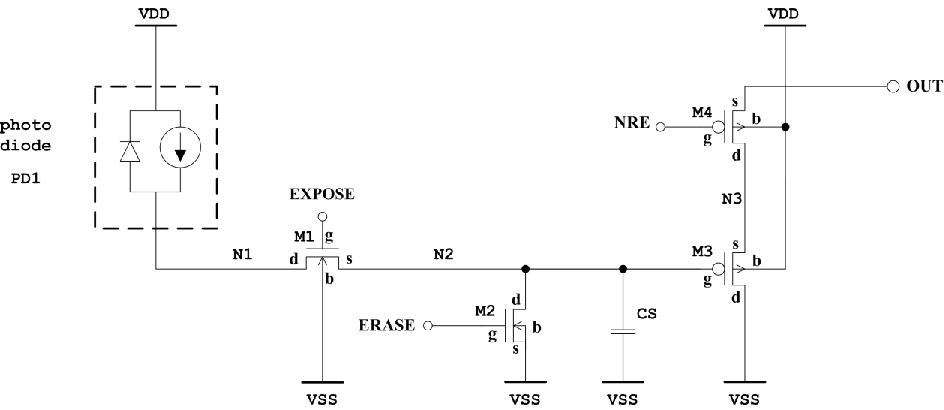
\includegraphics[width=\textwidth]{Images/Circuits/analog_circuit.pdf}
    \caption{Schematic of the analog readout part of the digital camera}
    \label{fig:system:an:sch}
\end{figure}

The analog part converts the electrons collected on the surface of the photodiode, in to an analog voltage. 
This voltage will charge up a capacitor depending on the lighting condition, for example low light condition will use longer time to charge capacitor. 
The expose transistor controls how  how long the capacitor can be charged for. 
The erase transistor controls the readout circuit so it does not overexpose the pixels. 
The two output transistors generate a current mirror which drives the output when a pixel is stored. 

To create a camera with more than one pixel, the pixels are connected in a matrix, shown in \cref{fig:app:fig:pixelarray} in \cref{fig:app:pixelarray}.

\subsection{Digital}

\begin{figure}[!htbp]
    \centering
    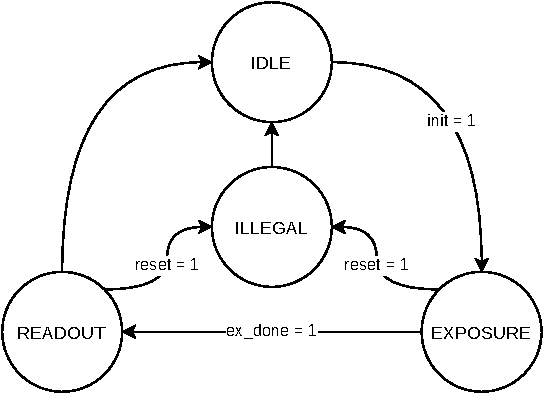
\includegraphics[width=0.7\textwidth]{Images/other/re_control_state.pdf}
    \caption{The different states of the control logic.}
    \label{fig:system:dig:states}
\end{figure}

The digital part controls the active pixel row, the exposure and the erase function of the analog part. 
%To obtain the required timing and the different states of capturing a picture, we use either a FPGA or an ASIC. 
%All three of these can be programmed by writing software with a HDL. 


From \cref{fig:system:dig:states} the four different states in the finite state machine (FSM) are presented. 
The FSM describes how the control logic captures a picture.
Starting with IDLE, the analog part is held stationary. 
When a picture is initialized, the state changes to EXPOSURE.
The pixels should be exposed for a set amount of time (until \texttt{ex\_done}, before continuing to the READOUT state. 
The READOUT consists of pulsing the pixel rows and controlling the ADC to read out the analog voltage to a digital value. 
After the readout is done, the state is set back to IDLE. 

The ILLEGAL state is used to reset the digital and analog parts, before going back to IDLE state.

All the timing of the FSM and states are synchronous, using a clock frequency of \SI{1}{\kilo\hertz}.

\clearpage
\section{Design process}
\subsection{Analog}
The analog part of the circuit was designed and verified using SPICE simulations in  AIM-SPICE. 
As the device models where provided, the task was to develop the SPICE nets and simulation stimuli.\\
To allow a low voltage drop over the transistors, the length of the NMOS transistors where picked to be as short as possible, while maintaining the project specification, as shown in \cref{tab:trans}. 
The width of the NMOS was therefore picked as wide possible. 
The PMOS transistors where picked to be equally as strong as the NMOS transistors. 
Therefore the PMOS lengths where picked to be equal, but the widths should be slightly larger due to the mobility relation between the transistors.

\begin{table}[!htbp]
    \centering
    \begin{tabular}{c|c|c}
        Transistor & L  & W \\\hline
        M1 & \SI{0.40}{\micro\meter} & \SI{1.20}{\micro\meter} \\
        M2 & \SI{0.40}{\micro\meter} & \SI{1.20}{\micro\meter} \\
        M3 & \SI{0.40}{\micro\meter} & \SI{4.63}{\micro\meter} \\ 
        M4 & \SI{0.40}{\micro\meter} & \SI{4.63}{\micro\meter}
    \end{tabular}
    \caption{Transistor dimension specifications}
    \label{tab:trans}
\end{table}

As both CC1 and CC2 where given, the only capacitor that had to be chosen was CS. The value of CS was picked to be large enough to be charged during exposure, as well as not being to large as that would reduce the speed of operation. Capacitor values are shown in \cref{tab:caps}.

\begin{table}[!htbp]
    \centering
    \begin{tabular}{c|c}
        Capacitor & Capacitance \\\hline
        CS  & \SI{2}{\pico\farad} \\
        CC1 & \SI{3}{\pico\farad} \\
        CC2 & \SI{3}{\pico\farad}
    \end{tabular}
    \caption{Capacitor specifications}
    \label{tab:caps}
\end{table}

\subsubsection{Corner analysis}
\label{Corn_analysis}
To demonstrate process variation, a simulation for an NMOS switch was done using AIMSPICE. 
The simulation covered some of the corner types mentioned in \cref{proc_var}. 
The following corners where simulated: TT, FF and SS.

\subsection{Digital}

The digital control logic is designed entirely with SystemVerilog, which is a superset of Verilog HDL.
\Cref{fig:system:dig:states} describes how the FSM in the control logic should behave, and \cref{fig:pros:dig:block} describes the top level logic block.

\begin{figure}[!htbp]
    \centering
    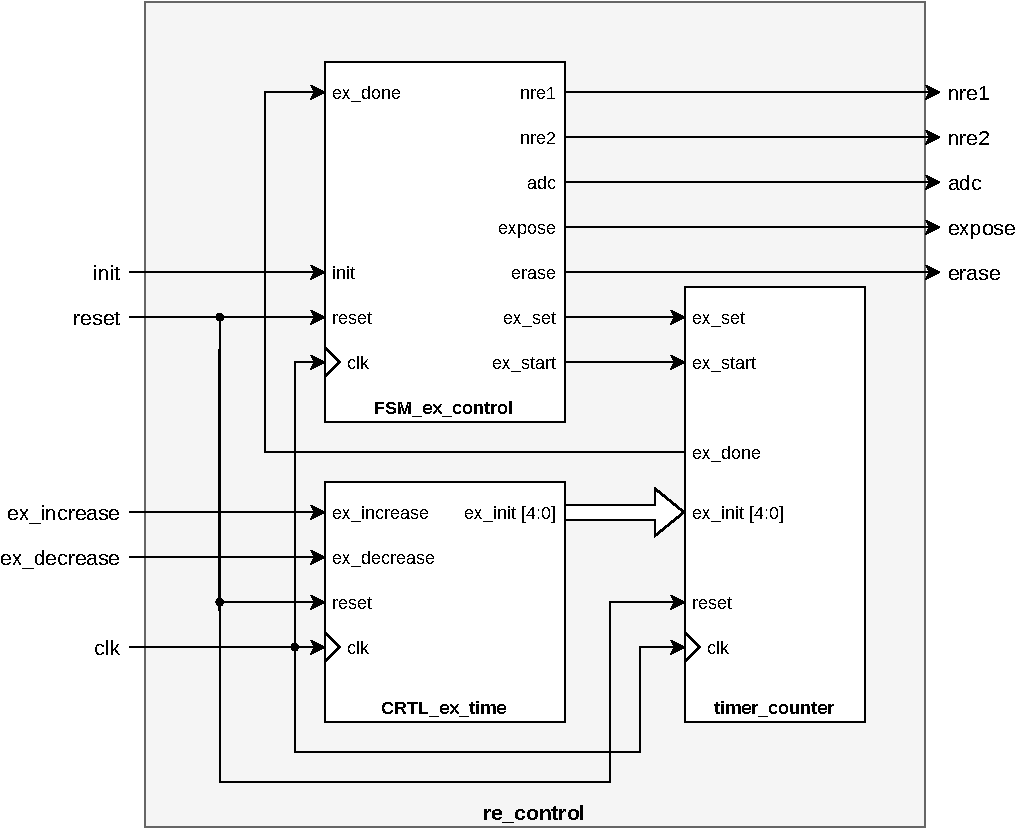
\includegraphics[width=.9\textwidth]{Images/Block_diagrams/re_control_block.pdf}
    \caption{Block diagram for the top level digital block. Top level contain the three smaller blocks that actually contain the logic.}
    \label{fig:pros:dig:block}
\end{figure}

There are three logic blocks inside the top level block, \texttt{FSM\_ex\_control}, \texttt{CTRL\_ex\_time} and\\ \texttt{timer\_counter}. 
The main control block and FSM is the \texttt{FSM\_ex\_control} block.
The FSM is implemented with a clock triggered switch statement. 
Each time this is triggered, it checks the current state, and operates according to what the state should do. 
When the FSM is in the EXPOSURE state, the two other blocks are used. 
The \texttt{CTRL\_ex\_time} block, only has a counter with how many milliseconds the exposure should last.
While \texttt{timer\_counter} uses a downward counting counter, to keep track of the exposure time. 
When done the \texttt{ex\_done} flag is set high, so that the FSM can continue to the next state which is READOUT.

In READOUT there is another smaller and simpler FSM, just to clock out the various control signals for the pixels and pixel array. 

When readout is done, the FSM returns back to the IDLE state.

The purpose of the ILLEGAL state is to ensure that all the control signals and the two other blocks are set to their proper stationary state. 
For instance if you are in the middle of an exposure, and suddenly trigging \texttt{reset} to 1. 
The ILLEGAL state will then ensure that the camera FSM can start properly from IDLE.




\clearpage
\section{Results}

The code for analog simulation is listed in \cref{app:analog}. 
Code for digital control logic is listed in \cref{app:digital}. 
All the plots were created with the MATLAB code in \cref{app:other:matlab}.

\subsection{Analog}
\label{Analog_res}
The analog readout circuit was simulated thoroughly with different exposure voltages to simulate multiple lighting conditions. 
In \cref{fig:res:anal:all@2ms} the simulation result at 2ms exposure time is presented. 
In the first and second plot pane the erase and exposure voltages are presented. 
Both of these voltages influence the sampled voltages which are presented in the third plot pane. 
This plot pane shows the behaviour of the capacitor at different photodiode currents 200pA, 250pA, 500pA and 750pA.
The Fourth plot pane shows the read enable transistor voltages in the same simulation. 
These are active low, meaning that they will have a voltage drop when activated. 
The final plot plane shows the circuit output voltages, which are thought to be sent to an ADC.

\begin{figure}[!htbp]
    \centering
    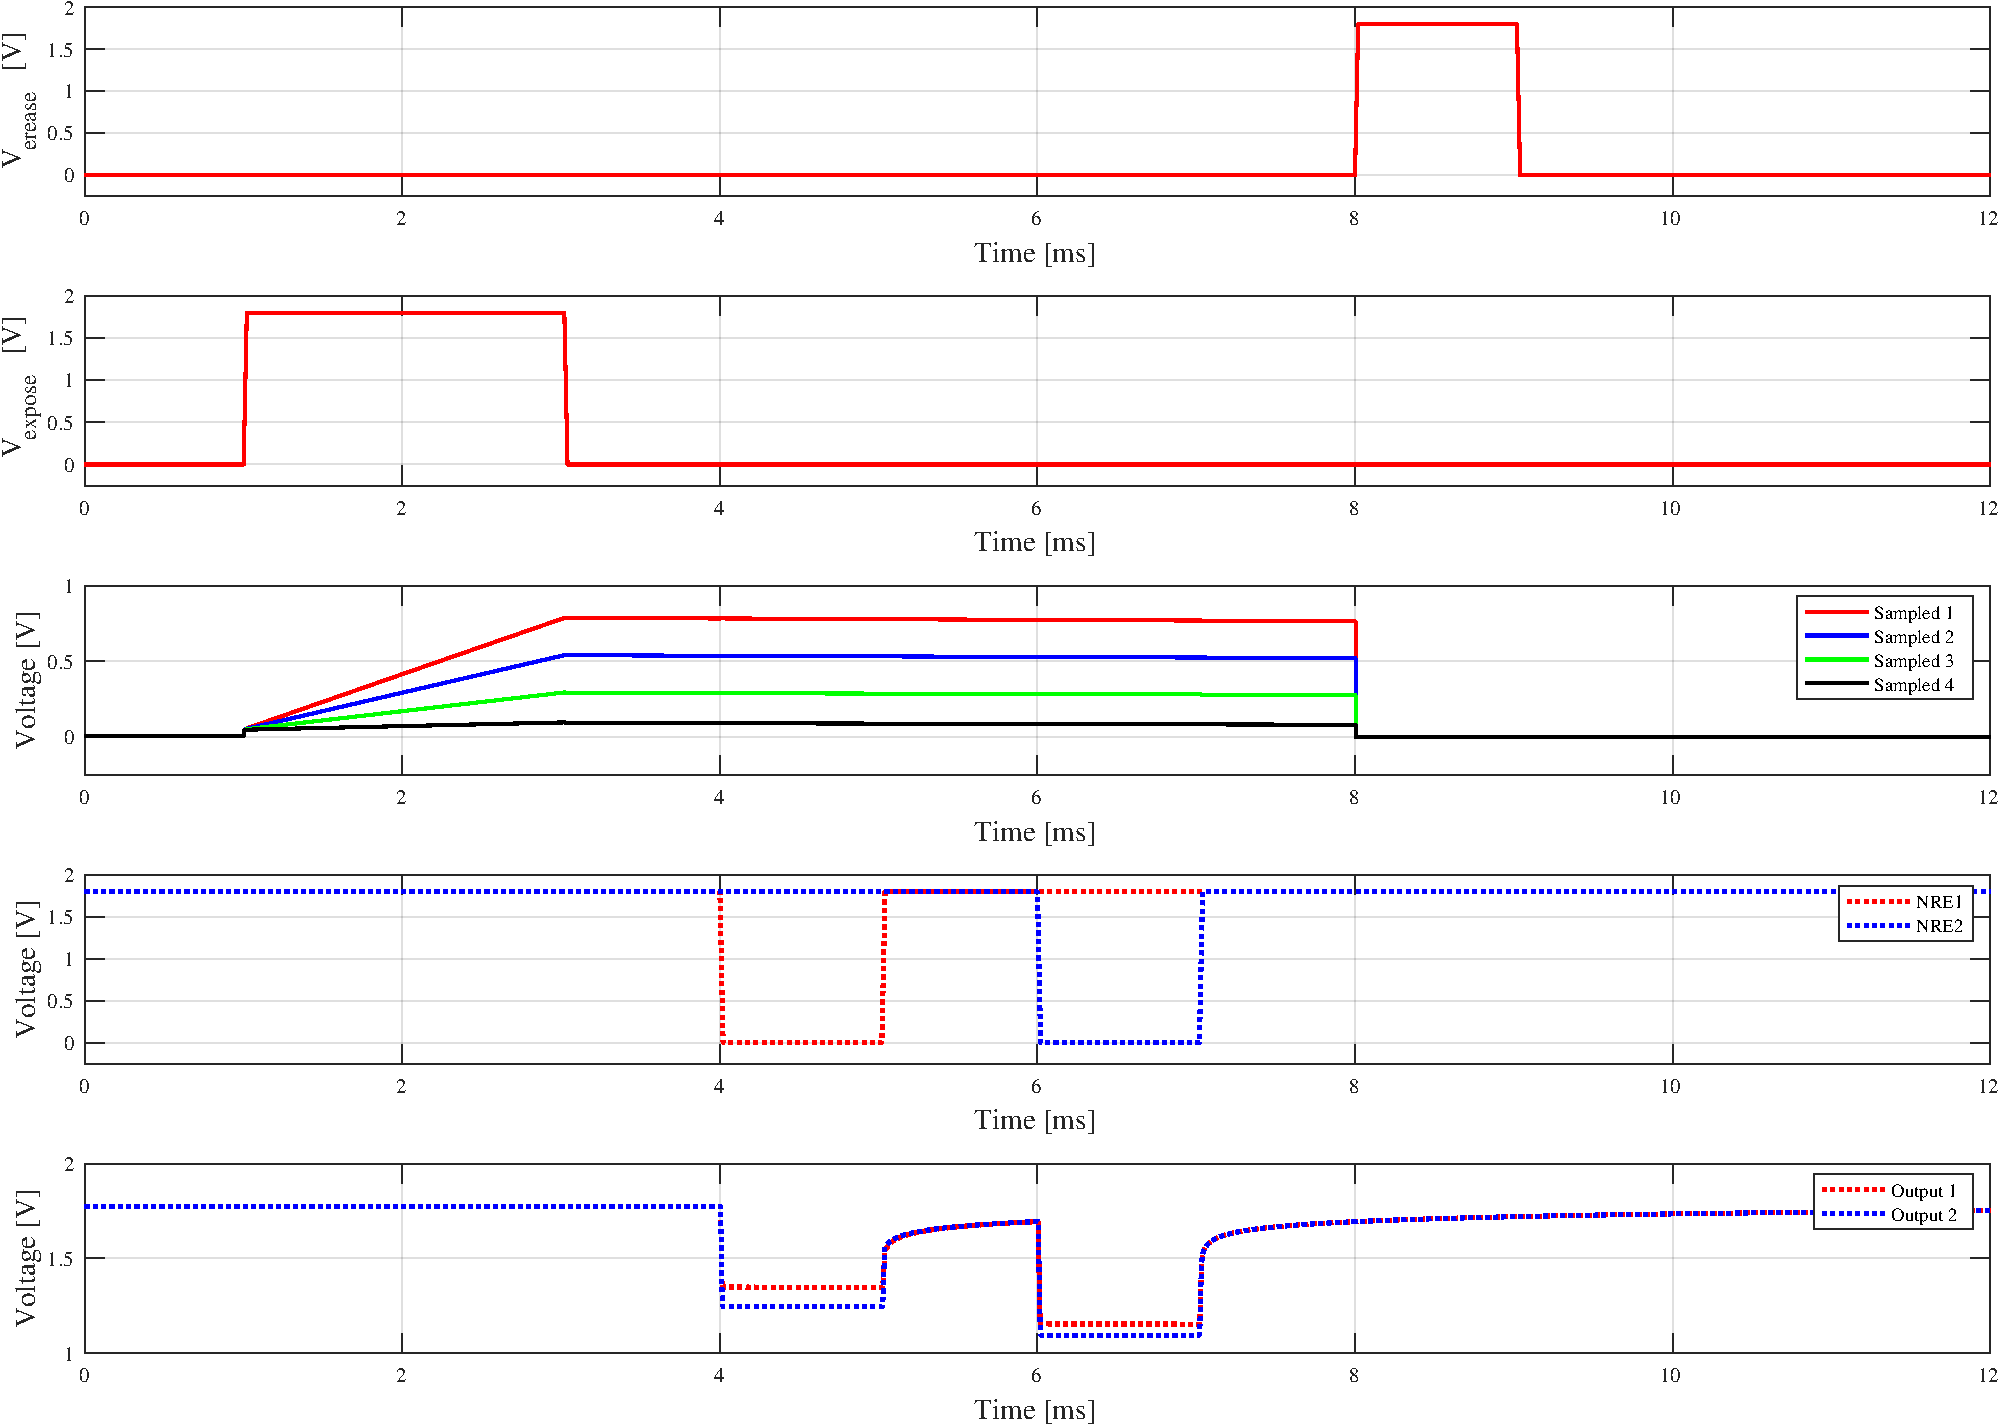
\includegraphics[width=\textwidth]{Images/Analog_plots/all_in_1.pdf}
    \caption{Node voltages at 2ms exposure time, under different photodiode currents}
    \label{fig:res:anal:all@2ms}
\end{figure}

The same node-voltages are simulated and plotted in \cref{fig:res:anal:all@30ms} at a longer exposure time of 30ms, where it shows that the lower photo diode currents will saturate the capacitor. 
The same photo diode currents as before are simulated here i.e. 200pA, 250pA, 500pA and 750pA.

\begin{figure}[H]
    \centering
    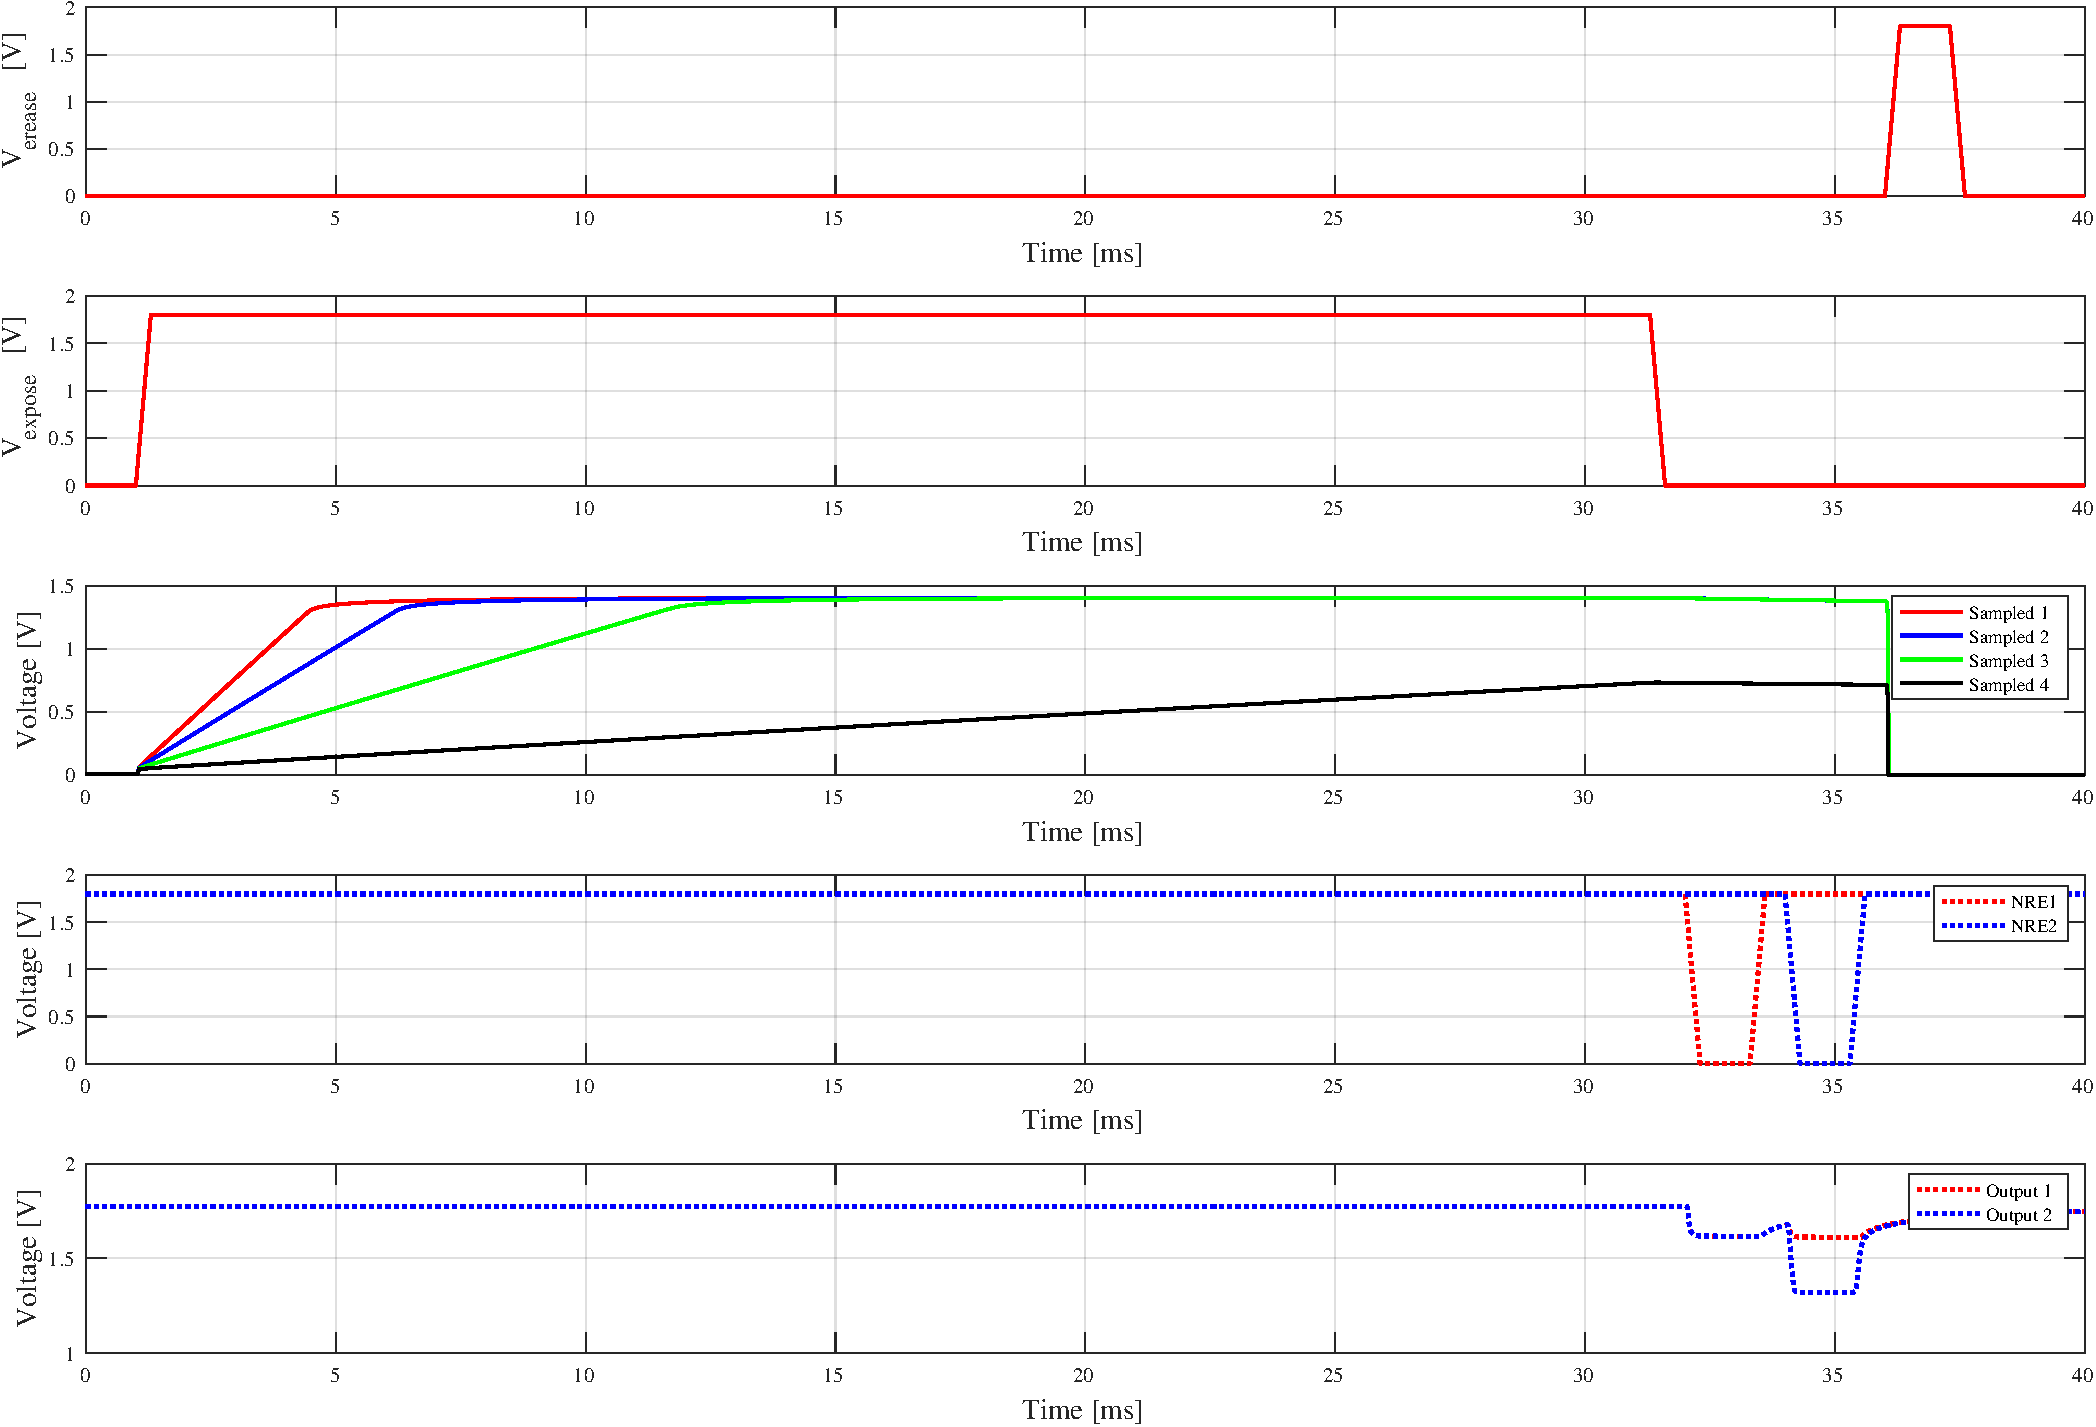
\includegraphics[width=\textwidth]{Images/Analog_plots/all_in_1@30ms.pdf}
    \caption{Node voltages at 30ms exposure time, under different photodiode currents}
    \label{fig:res:anal:all@30ms}
\end{figure}

\Cref{fig:res:anal:all2} shows the same simulation as \cref{fig:res:anal:all@2ms}, but a closer look at the capacitor voltage response to the exposure voltage and erase voltage. 
It shows that the exposure voltage charges the capacitor up to a certain voltage potential, dependent on the diode current and exposure time. 
It also shows that when the erase transistor receives its voltage, the capacitor discharges, and is ready for a new exposure. 

\begin{figure}[H]
    \centering
    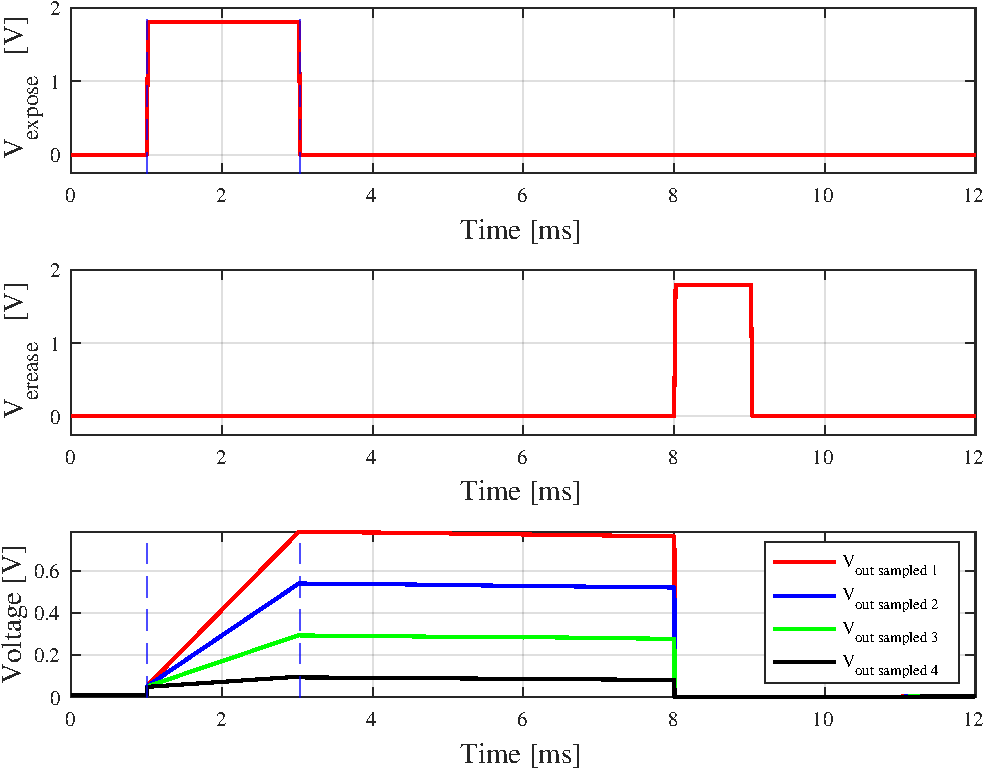
\includegraphics[width=\textwidth]{Images/Analog_plots/exp_eras_sample_m_voltage.pdf}
    \caption{Capacitor voltages vs. control voltages}
    \label{fig:res:anal:all2}
\end{figure}

\Cref{fig:res:anal:all3} shows a closer look at the capacitor voltages at 2ms exposure under the four different lighting conditions, i.e. diode currents.

\begin{figure}[H]
    \centering
    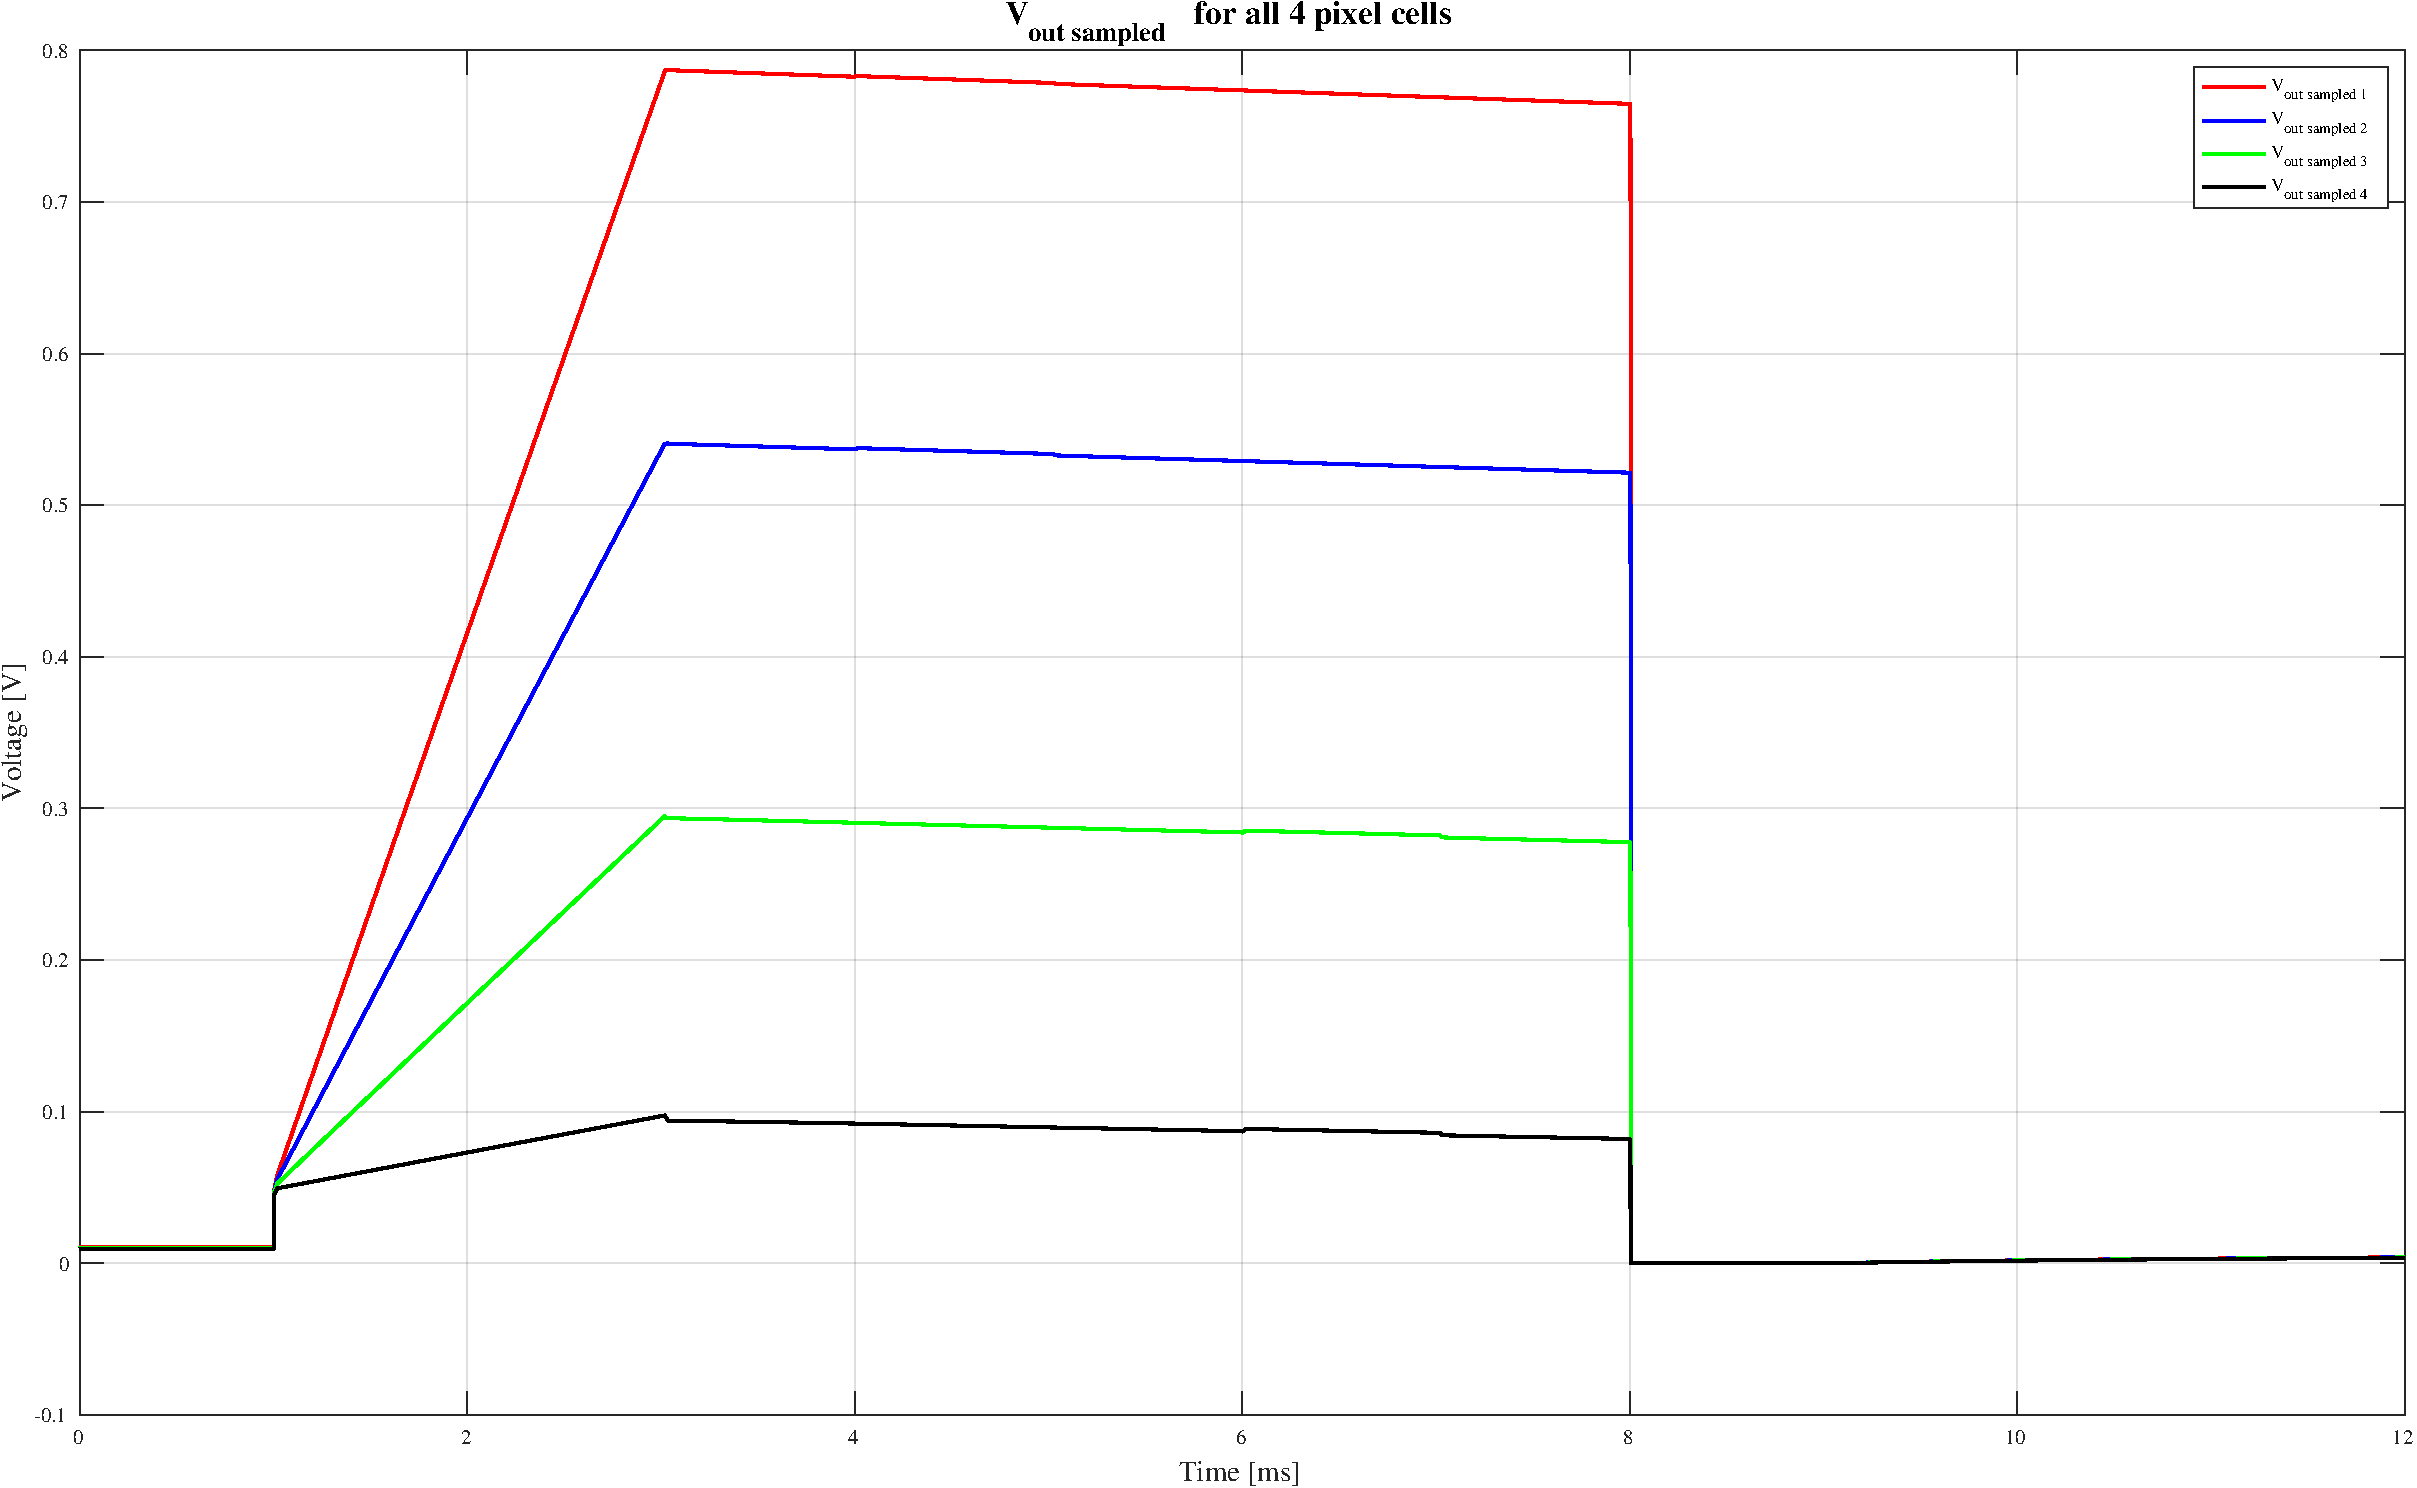
\includegraphics[width=\textwidth]{Images/Analog_plots/v_out_sampled_all_2ms.pdf}
    \caption{Capcitor voltages under different lighting conditions at 2ms exposure time}
    \label{fig:res:anal:all3}
\end{figure}


\subsubsection{Corner analysis}
As mentioned in \cref{Corn_analysis}, a corner analysis of an NMOS switch was done. 
The transconductance of an NMOS where plotted using three different process corners, TT, FF and SS. 
The SPICE net used for this simulation is included in \cref{app:switch}

\begin{figure}[H]
    \centering
    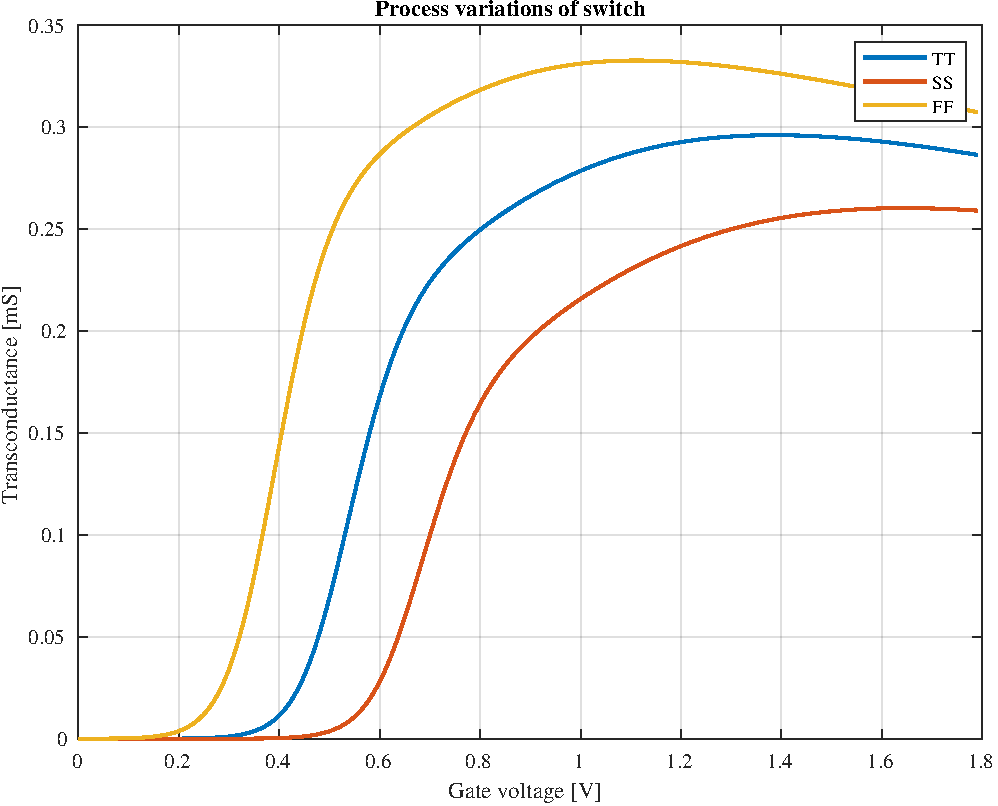
\includegraphics[width=\textwidth]{Images/Analog_plots/corneranalysis.pdf}
    \caption{Corner analysis of NMOS switch}
    \label{fig:res:anal:corn_nmos}
\end{figure}


\subsection{Digital}

All verilog code was compiled with Icarus Verilog \cite{williams_2020}, \mintinline{bash}{iverilog}. 
To compile with SystemVerilog 2005 use the flag \mintinline{bash}{-g2005-sv}.

\Cref{fig:res:dig:timer} shows the timing diagram for the \texttt{timer\_counter} block.
To set the initial value to count from, it is shown set the \texttt{ex\_set} high.
When \texttt{ex\_start} is set high the timer start counting down to $0$.
When it reaches $0$ the signal \texttt{ex\_done} is set high.

\begin{figure}[!htbp]
    \centering
    \fbox{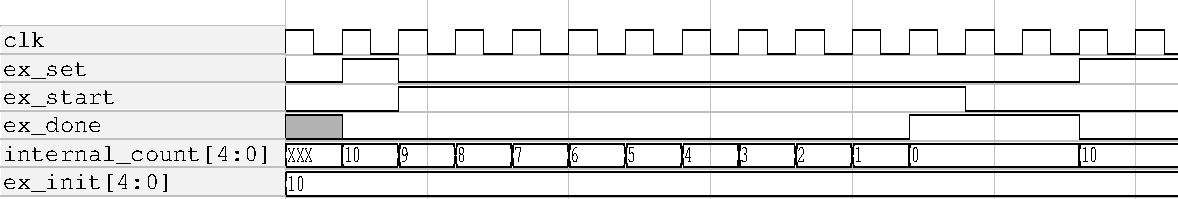
\includegraphics[width=.95\textwidth]{Images/Digital_plots/timer_counter_tb.pdf}}
    \caption{Timing diagram for the \texttt{timer\_counter} block. Larger version in \cref{app:figs:timer_counter}}
    \label{fig:res:dig:timer}
\end{figure}

\Cref{fig:res:dig:CTRL} shows the timing diagram for the \texttt{CTRL\_ex\_time} block.
When \texttt{ex\_increase} is set high, it will increase the exposure time by one for each clock cycle.
Similar for \texttt{ex\_decrease}, but it decreases the exposure time. 

There is a maximum and minimum value of 30 ms and 2 ms respectively. 
Both inc/decrease and the limits are tested and shown in \cref{fig:res:dig:CTRL}.
When \texttt{reset} is set high, the initial value is set to $16$, which is in the middle of $30$ and $2$.

\begin{figure}[!htbp]
    \centering
    \fbox{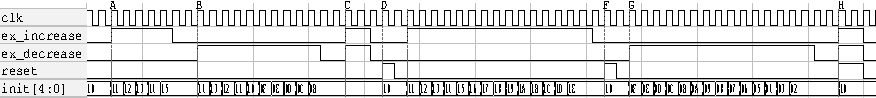
\includegraphics[width=.95\textwidth]{Images/Digital_plots/CTRL_ex_time_tb.pdf}}
    \caption{Timing diagram for the \texttt{CTRL\_ex\_time} block. Larger version in \cref{app:figs:CTRL}}
    \label{fig:res:dig:CTRL}
\end{figure}

In \cref{fig:res:dig:FSM}, the timing diagram for the main logic block, \texttt{FSM\_ex\_control}, is shown.
The FSM is reset when \texttt{reset} is high. This happens at \texttt{A}. At \texttt{B} we have a state change into EXPOSING. This is done until \texttt{ex\_done} is set high. 
When this happens at \texttt{C}, the state is set to READOUT, and the readout sequence for the pixel array is initiated. 
At \texttt{D} and \texttt{E} the FSM returns to the IDLE state, finishing the sequence of capturing a picture.

\begin{figure}[!htbp]
    \centering
    \fbox{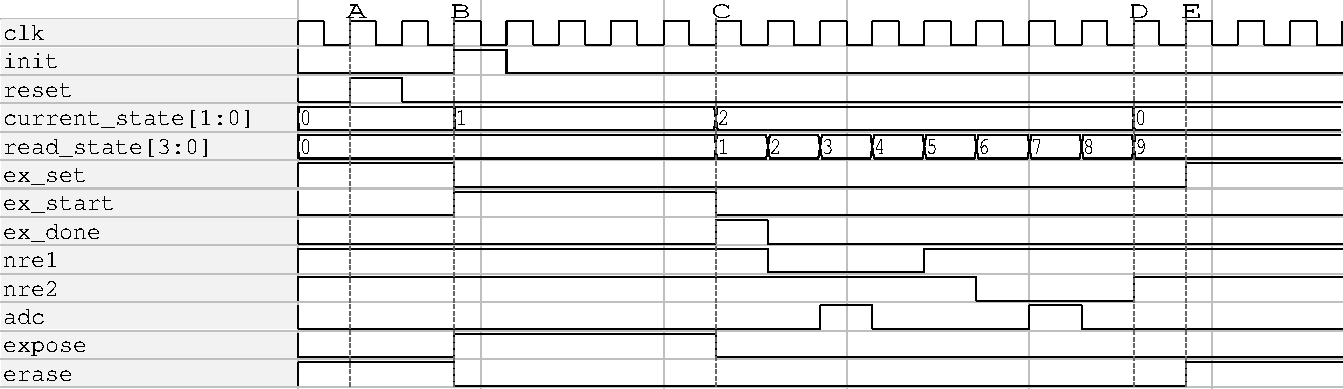
\includegraphics[width=.95\textwidth]{Images/Digital_plots/FSM_ex_control_tb.pdf}}
    \caption{Timing diagram for the \texttt{FSM\_ex\_control} block. Larger version in \cref{app:figs:FSM}}
    \label{fig:res:dig:FSM}
\end{figure}

\Cref{fig:res:dig:re_control} is the combined timing diagram for the top level block, \texttt{re\_control}. 
When resetting at \texttt{A}, we can continue by decreasing the exposure time at \texttt{B}.
This is done until we have 10 ms exposure. At \texttt{C}, we initiate the capture sequence by exposing and starting the exposure counter.
At \texttt{D} the exposure is done, 10 clock cycles later than initialization (at 1kHz that is 10ms).
Following is the readout, same as in \cref{fig:res:dig:FSM}. 
At \texttt{E} the sequence is done and all values are set back to the initial values and the state is set to IDLE.

\begin{figure}[!htbp]
    \centering
    \fbox{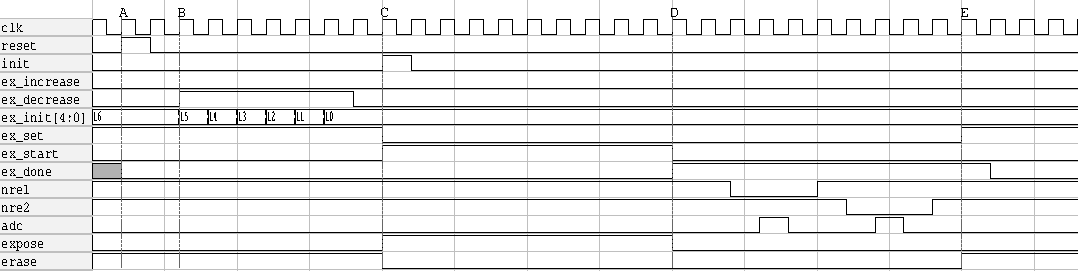
\includegraphics[width=.95\textwidth]{Images/Digital_plots/re_control_tb.pdf}}
    \caption{Timing diagram for the \texttt{re\_control} block. Larger version in \cref{app:figs:re_control}}
    \label{fig:res:dig:re_control}
\end{figure}

\clearpage
\section{Discussion}
\subsection{Analog}
Although the simulations presented in \cref{Analog_res} seems quite promising. 
Seeing as the capacitor gets charged at the different voltages under the different simulated lighting conditions. 
As well as being discharged when the erase transistor gets activated. 
The circuit has yet to be tested simulated in a mixed signal simulation. 
The SPICE simulations have "hard" coded control signals to simulate the digital control, meaning that the interface between the two parts has yet to be tested.

\subsubsection{Corner analysis}
The process variations are not simulated on the complete analog circuit, only on a single NMOS switch. 
Therefore there is no reason to rule out that process variations may affect the function and performance of the analog circuit.

\subsection{Digital}
The digital circuit seems to function after the specification, this means that it works under the same timing as the analog circuit does. 
However since the verilog HDL is only synthesized and simulated in software and has yet to be implemented in hardware, there is no guarantee that a hardware implementation will work as simulated.

\clearpage
\section{Conclusion}
Since all simulation results function after specification, the digital camera module is at least theoretically accomplished. 
Both the analog and digital parts of the system works individually, but has yet to be simulated together in a mixed signal analysis. 
A simulation tool supporting both analog and digital mixed signal analysis should be used to test this functionality.

Seeing as the module has only been simulated, it is still only theoretically accomplished and has yet to be implemented in hardware. 
The process variations of the analog circuit may affect a hardware implementation. 
A hardware implementation of the digital circuit may also not work as the simulations shows.




% Example section added directly into the main-file


% Printing bibliography
\newpage
\printbibliography[heading = bibintoc, title = Bibliography]    % 'bibintoc' inserts our bibliography into the table of contents

% Inserting appendix with separate settings
\addappendix
\import{./Appendices/}{figures}
\clearpage
\import{./Appendices/}{analog}
\clearpage
\import{./Appendices/}{digital}
\clearpage
\import{./Appendices/}{other}

% End of document
\end{document}
